\section{Modulation}
\subsection{Grundbegriffe}
Es gibt grundsätzlich drei Arten von Modulation für Sinus/Cosinussignale welche in den nachfolgenden Kapitel genauer erläutert werden.\script{40}
\begin{itemize}[nosep]
	\item Amplitudenmodulation (AM) - Kapitel \ref{AM}
	\item Phasenmodulation (PM) - Kapitel \ref{PM}
	\item Frequenzmodulation (FM) - Kapitel \ref{FM}
\end{itemize}
~\\
\noindent Für Rechteckssignale gibt es desweiteren \script{41}
\begin{itemize}[nosep]
	\item Pulsamplitudenmodulation (PAM)
	\item Pulsweitenmodulation (PWM)
	\item Pulspositionmodulation (PPM)
	\item Pulsfrequenzmodulation (PFM)
\end{itemize}

\subsection{Basisbanddarstellung}
Die Basisbanddarstellung zeigt alle möglichen Werte des modulierten Signals. Für AM (Siehe auch \script{49}) variiart die Amplitude, Phase ist aber Konstant. Daher resultiert eine gerade. Bei Winkelmodulation umgekehrt, die Amplitude ist konstant und Phase variiart, was ein Kreissegment ergibt. Wenn mit der Bessel-Summe das $\beta$ bestimmt ist ergibt dies den Winkel.
~\\
Dafür wird das komplexe Signal in Realteil und Imaginarteil aufgeteilt und entsprechnd im Zeigerdiagramm dargestellt.~\\

\noindent\textbf{Beispiel AM} für $\mu = 25\%$ und $A_c=1$ und normiertem Nachrichtensignal $|m(t)| \leq 1$:
\begin{align*}
	x_{AM}(t) &= A_c \cdot (1 + \mu m(t)) \cdot \cos(\omega_ct) \\
	&= A_c \cdot (1 + \mu m(t)) \frac{1}{2}(e^{j\omega_ct} + e^{-j\omega_ct})
\end{align*}
\begin{align*}
	\Im[x_{AM}(t)] &= 0\\
	\Re[x_{AM}(t)] &=  A_c \cdot (1 + \mu m(t))\qquad \in [0.75, 1.25]
\end{align*}

\begin{center}
	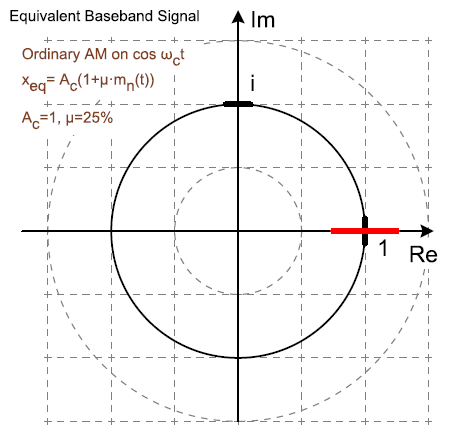
\includegraphics[width=0.5\columnwidth]{Images/orinary_am_eq}
\end{center}


\noindent\textbf{Beipiel PM} für $\beta = 0.6rad$ und $A_c = 1$:
\begin{center}
	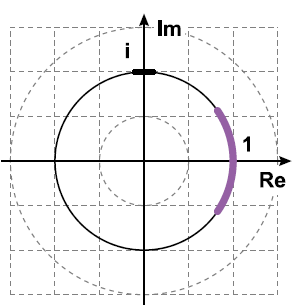
\includegraphics[width=0.5\columnwidth]{Images/phim_eq}
\end{center}

\subsection{Amplitudentmodulation - AM}\label{AM}\script{39}
Bei der Amplitudentmodulation ist die Amplitude des Trägersignals $x_c(t)$ linear von dem Nachrichtensignal $m(t)$ abhängig.

\begin{tabular}{lll}
	Trägersignal & carrier & $x_c(t) = A_c \cdot \cos(\omega_ct)$ \\
	Nachrichtensignal & message & $m(t)$ \\
\end{tabular}


\subsubsection{OAM}\script{45}
Ordinary Amplidutdenmodulation (Gewöhnliche AM) mit $\mu \in [0, 1] = \frac{\left|\min m(t)\right|}{A_c}$ als \textbf{Modulationsgrad} und Nachrichtensignal $m_n(t)$. 

Ziel ist es mit der Skalierung sicherzustellen, dass keine Negativen Werte mit der Modulation entstehen, da ansonsten die Demodulation schwierig wird. 
\begin{align*}
	x_{AM}(t) &= A_c (\overbrace{1 + \mu \cdot m_n(t)}^{\text{Skalierung}})\cdot\cos(\omega_ct) \\
	X_{AM}(\omega) &= \pi A_c (\delta(\omega - \omega_c) + \delta(\omega + \omega_c)) \\
	& + \frac{\mu A_c}{2}(M_n(\omega - \omega_c) + M_n(\omega + \omega_c))
\end{align*}
\noindent\textbf{Achtung:} Trägersignal im Frequenzbereich $\cos$ ~\\

\noindent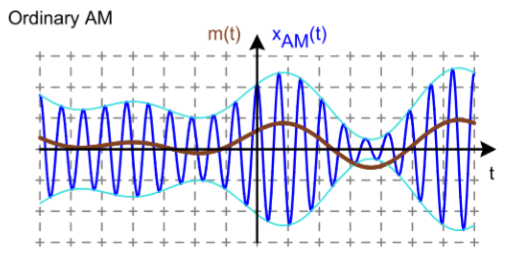
\includegraphics[width=0.4\columnwidth]{Images/oam} 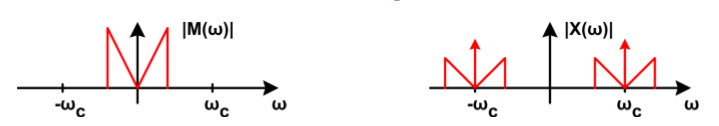
\includegraphics[width=0.6\columnwidth]{Images/oam_f}\\

\noindent Speziell bei der OAM, es wird immer ein DC-Anteil (zB hier $+1$) hinzugefügt, welche im Frequenzbereich herausgelesen werden kann (Dirac-Stoss). Im Zeitbereich ergeben sich dadurch keine Negativen Werte. ~\\

\noindent Die \textbf{Bandbreite} $B_m$ des Nachrichtensignals wird  verdoppelt: $B_{AM} = 2\cdot B_m$\\ ~\\
\noindent Die \textbf{Leistung} $P_{AM} = \frac{A_c^2}{2}\cdot(\overbrace{1}^{P_{DC}} + \mu^2 + m_{rms}^2)$. Daraus kann die \textbf{Leistungseffizienz} $\eta = \frac{P_{sb}}{P_{AM}} = \frac{\left(\frac{\mu}{C}\right)^2}{1+\left(\frac{\mu}{C}\right)^2}$ von OAM bestimmt werden \script{50}. Wobei $C$ der Crestfaktor ist.

\subsubsection{DSB-SC}\script{51}
Double-sideband suppressed-carrier hat, im unterschied zu OAM, kein DC-Anteil (Dirac-Stoss) und die gesammte Leistungseffizient in den Seitenbändern. Das Nachrichtensignal wird bei der Modulation zum Trägersignal hin verschoben ($\pm \omega_c$). Bei der Demodulation wird dies wiederholt, was zusammen mit einem LPF das Ursprüngliche Nachrichtensignal wieder ergibt.
\begin{align*}
	x_{DSB}(t) &= A_c \cdot m_n(t)\cdot\cos(\omega_ct) \\
	X_{DSB}(\omega) &= \frac{A_c}{2}\cdot(M_n(\omega - \omega_c) + M_n(\omega + \omega_c))
\end{align*}

\noindent\textbf{Achtung:} Trägersignal im Frequenzbereich $\cos$ ~\\

\noindent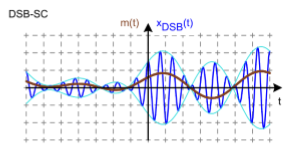
\includegraphics[width=0.4\columnwidth]{Images/dsb_sc} 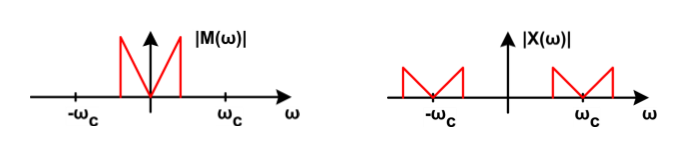
\includegraphics[width=0.6\columnwidth]{Images/dsb_sc_f} \\

\noindent Speizell bei DSB-SC, es hat im Zeitbereich auch Negative Werte. Im Frequenzbereich ist kein DC-Anteil zu sehen. Die \textbf{Bandbreite} $B_{DSB-SC}$ mit maximaler Frequenz des Nachrichtensignals $f_m$ ist $B_{DSB-SC} = 2 \cdot f_m$. Die Leistung ist gegeben durch $P_{DSB} = \frac{A_c}{2}\cdot P_m$.

\subsubsection{SSB}\script{53}
Single-Sideband modulation. Wenn Nachrichtensignal $m_n$ Reellwertig ist, dann kann die Negative Frequenzachse weggelassen werden, da diese Konjugiert-Komplex sein müssen. Wobei $\hat{m}_n$ die Hilbert-Transformierte Kapitel \ref{hilbert} von dem Nachrichtensignal ist.

\begin{align*}
	x_{SSB} &= A_c \cdot m_n(t) \cdot \cos(\omega_ct) \mp A_c\cdot \hat{m}_n\cdot \sin(\omega_ct) \\
	X_{DSB}(\omega) &= \frac{A_c}{2}\cdot(M_n(\omega - \omega_c) + M_n(\omega + \omega_c))
\end{align*}

\noindent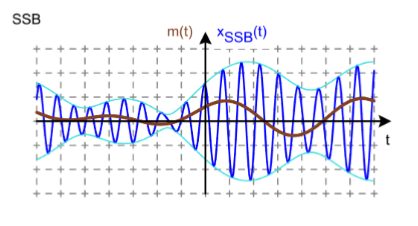
\includegraphics[width=0.3\columnwidth]{Images/ssb} 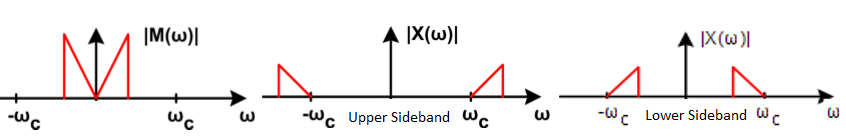
\includegraphics[width=0.7\columnwidth]{Images/ssb_f}\\ 

\noindent Die \textbf{Bandbreite} $B_m$ des Nachrichtensignals bleibt erhalten: $B_{SSB} = B_m$

\subsubsection{VSB}\script{57}
Restseitenband-Amplidudenmodulation. Eine Seitenband wird komplett, das zweite mit reduzierter Bandbreite Übertragen. Kompromisslösung zwischen SSB und DSB-SC.


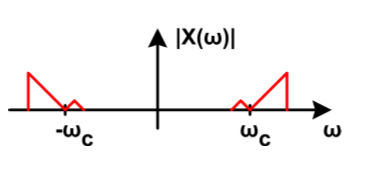
\includegraphics[width=0.7\columnwidth]{Images/vsb}\\

\subsubsection{QAM}\script{57}
Quadraturamplitudenmodulation überlagert zwei komplett unabhängige (aber orthogonal zueinander) modulierte DSB-SC Signale.

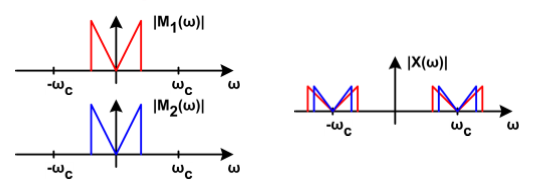
\includegraphics[width=0.7\columnwidth]{Images/qam}\\

\noindent Die \textbf{Bandbreite} $B_m$ des Nachrichtensignals wird verdoppelt: $B_{QAM} = 2\cdot \max(B_{m_1}, B_{m_2})$\\ ~\\
\noindent Die \textbf{Leistung} $P_{QAM} = P_{DSB_1} + P_{DSB_2}$.


\subsection{Winkelmodulation}
Obwohl Winkelmodulationen - im vergleich zu AM - komplexer und mehr Bandbreite benötigen, hat es den erheblichen Vorteil, dass \textbf{Störanfolligkeiten} und \textbf{Rauschen} kleiner als bei AM sind.

Die Grundlage bietet der sinusförmige Träger, wessen Phase oder Frequenz je nach Amplitude des Nachrichtensignals moduliert wird:
\[
x_c(t) = A_c \cdot \cos(\overbrace{\omega_ct + \varphi(t)}^{\theta(t)})
\]

\noindent Die \textbf{Leistung} kann bei PM/FM sehr genau mit $P = \frac{A_c^2}{2}$ abgeschätzt werden.\\
\noindent Die \textbf{Bandbreite} $B_{\varphi m}$ des Nachrichtensignals wird mindestens $B_{\varphi m} \geq 2\cdot B_m$\\ ~\\
\subsubsection{Phasenmodulation}\label{PM}\script{60}
Die Phasenmodulation im Zeitbereich, wobei $k_p$ die Phasenhubkonstante in [rad] und $\varphi(t)$ die \textbf{momentan Phasenabweichung} ist.
\begin{align*}
x_{PM}(t) &= A_c\cdot \cos(\omega_ct + \varphi(t)) \qquad \varphi(t) = k_p\cdot m(t)
\end{align*}

\begin{center}
	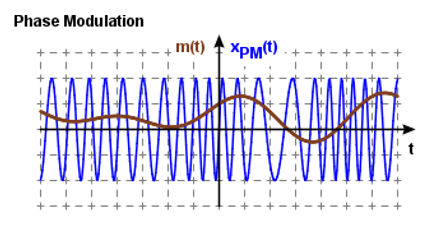
\includegraphics[width=0.6\columnwidth]{Images/pm}
\end{center}

\noindent momentane \textbf{Kreisfrequenzabweichung} $\frac{d\varphi(t)}{dt} = k_p \cdot \frac{dm(t)}{dt}$\\ \noindent momentane \textbf{Kreisfrequenz} $\omega_c + \frac{d\varphi(t)}{dt} = \omega_c + k_p\cdot \frac{dm(t)}{dt}$.

\subsubsection{Frequenzmodulation}\label{FM}\script{60}
Die Frequenzmodulation im Zeitbereich wobei $k_F$ die Frequenzhubkonstante in [rad/s] und $\varphi(t)$ die \textbf{momentane Phasenabweichung} ist.
\begin{align*}
	x_{FM} = A_c\cdot\cos(\omega_ct + \varphi(t)) \qquad \frac{d\varphi(t)}{dt} &= k_F\cdot m(t) \\
	\varphi(t) &= k_F\int_{-\infty}^{t}m(\tau)d\tau
\end{align*}

\begin{center}
	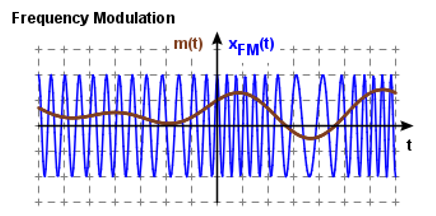
\includegraphics[width=0.6\columnwidth]{Images/fm}
\end{center}

\noindent momentane \textbf{Kreisfrequenzabweichung} $\frac{d\varphi(t)}{dt} = k_F \cdot m(t)$\\ 
\noindent momentane \textbf{Kreisfrequenz} $\omega_c + \frac{d\varphi(t)}{dt} = \omega_c + k_F\cdot m(t)$.
~\\ ~\\
\noindent\textbf{Beispiel}\\
Momentanfrequenz $\omega_i(t)$ bei Phasen-und Frequenzmodulation ist die Ableitung des Argumentes $\theta$ vom Trägersignal.\\ $x_{FM}(t) = 10\cos(\underbrace{200\pi t + \pi t^2}_\theta) \xrightarrow{\omega_i(t) = \frac{d\theta}{dt}} \omega_i(t) = 2\pi (10 + t)$

\subsection{Kleinhub}\script{62}
Die Idee von Narrowband Angle Modulation ist, dass die nicht-linearen Terme von $\varphi(t)$ verschwindend klein bleiben. Dies glit bis ca. $\varphi(t) < 0.2rad \approx 12^\circ$. Die Leistungseffizienz $\eta$ kann mit AM approximiert werden.

\subsection{Grosshub}\script{63}
Bei Grosshubsignalen kannen die nicht-linearen Terme in $\varphi(t)$ nicht mehr vernachlässigt werden. Dadurch entstehen neue Frequenzkomponenten, welche die Bandbreite des modulierten PM-/FM-Signal erhöht. Eine analytische Bestimming des Spektrum für komplexe Signale ist daher nicht mehr möglich. ~\\

\subsubsection{Einton-Winkelmodulation}
Für Eintonsignale, d.h für Sinusförmige Signale (oder auch Single-Tone Modulation) h kann eine Grosshubwinkelmodulation dennoch bestimmt werden.
\[
x_{ST\varphi M}(t) = A_c\cdot \cos(\omega_ct + \beta\cdot \sin(\omega_mt))
\]

\textbf{Beispiel:}\\
\begin{align*}
	x(t) &= \underbrace{10}_{A_c}\cos(\underbrace{2\pi10^8}_{\omega_c}t+\underbrace{200}_{\beta}\cos(\underbrace{2\pi10^3}_{\omega_m}t)) \\
	\xrightarrow{\text{W.mod}} B_{ST\varphi M} &= 2(200+1)\cdot 2\pi 10^3 / 2 \pi = 402kHz
\end{align*}


\subsubsection{Carson Bandbreite}\script{67}
Die Bandbreite $B_{ST\varphi M}$ eines Einton-Signals kann Abgeschätzt werden mit Carson:
\[B_{ST\varphi M} = 2(\beta + 1)\cdot\frac{\omega_m}{2\pi}\]

\noindent Dabei muss zwischen FM und PM unterschieden werden:
\begin{align*}
	B_{PM} &= 2(k_pA_m+1)\cdot\frac{\omega_m}{2\pi} \qquad \beta = k_p A_m \\
	B_{FM} &= 2\cdot\frac{\omega_mA_m + \omega_m}{2\pi} \qquad \beta = \frac{k_p A_m}{\omega_m}
\end{align*}

~\\
Die Maximale Phasenabweichung $\beta$ eines Eintonsignals kann auch mit der Frequenz des moulierenden Signals $f_m = \frac{\omega_m}{2\pi}$ und dem \textbf{Frequenzhub} (gibt an, um welche Frequnz sich das modulierte Signal von der Trägerfrequenz unterscheidet) $\Delta f = \frac{\Delta \omega}{2\pi}$ ausgedrückt werden, was speziell für FM-Signale folgende praktische Formal ergibt
\[\beta = \frac{\Delta\omega}{\omega_m} = \frac{\Delta f}{f_m}\]
Durch einsetzen der Carson-Bandbreite erhählt man:
\[B = 2(\Delta f + f_m)\]

\noindent Für Hubverhältnis siehe \script{67}

\subsubsection{Besselfunktion}
\[
x_{ST\varphi M}(t) = A_c \cos(\omega_ct+\beta\sin(\omega_mt)) = A_c \Re[e^{j\omega_ct} \cdot e^{j\beta\sin(\omega_mt)}]
\]


\begin{center}
	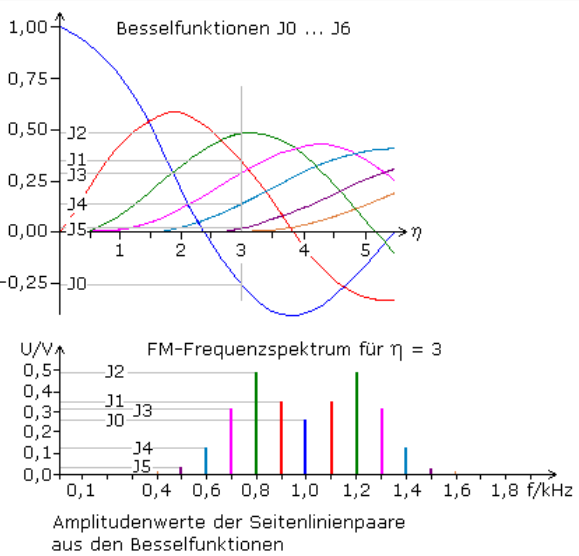
\includegraphics[width=0.8\columnwidth]{Images/besselfunktion}
\end{center}

Maximaler Phasenhub $\max(\varphi(t)) = \beta = k_p\cdot A_m$.~\\ \\


